\documentclass{article}
%
% Demo of the mcode package from 
% http://www.mathworks.co.uk/matlabcentral/fileexchange/8015-m-code-latex-package
% Updated 06 Mar 2014
%

\usepackage{graphicx}
\usepackage{wrapfig}
\usepackage{mathtools}
\usepackage{mathrsfs}
\usepackage{enumitem}
\usepackage{pdflscape}
\graphicspath{ {images/} }

% load package with ``framed'' and ``numbered'' option.
\usepackage[framed,numbered,autolinebreaks,useliterate]{mcode}

% something NOT relevant to the usage of the package.
\usepackage{url}
\setlength{\parindent}{0pt}
\setlength{\parskip}{18pt}


% //////////////////////////////////////////////////

\begin{document}

\title{Homework 3 - Optimal Control Systems}
\author{Erivelton Gualter dos Santos, 2703806}
\date{}

\maketitle 

\begin{wrapfigure}{l}{0.3\textwidth}
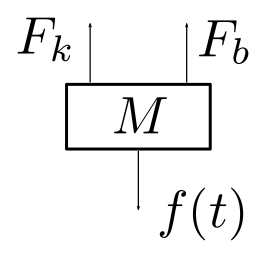
\includegraphics [width=1in]{output}
\caption{Free-Body Diagram for Exercise 1.3 - Kirk.}
\end{wrapfigure} 

\begin{enumerate}[]
\item Discretize the system of Kirk Problem 1.3. Compare your continuous-time and discrete-time simulation outputs to verify that you discretized it correctly.
\end{enumerate}

The following figure describes the free-body diagram. The governing equation for this system is:

\begin{equation*}
\ddot{y} = \frac{f - Ky - B\dot{y}}{M}
\end{equation*}

Defining the \textit{States Variables} $x_1$ and $x_2$ as $y$ and $\dot{y}$ respectively, we have: 
\begin{eqnarray}\label{i1}
\begin{split}
	\dot{x_1} &= x_2 \\
	\dot{x_2} &= -\frac{K}{M}x_1 -\frac{B}{M}x_2 +\frac{1}{M}f
\end{split}
\end{eqnarray}
Assuming that $M = 1\:kg$, $K = 2\:\frac{N}{m}$ and $B = 2\:\frac{N}{m/s}$, we have:
\begin{eqnarray}\label{i1}
\begin{split}
	\dot{x_1} &= x_2 \\
	\dot{x_2} &= -2x_1 -2x_2 + f
\end{split}
\end{eqnarray}

Recalling that: 
\begin{eqnarray}
\frac{x\left(t+\Delta t \right) -x(t)}{\Delta t} \approx a\left(x(t), u(t)\right)
\end{eqnarray}

Therefore, $x_n$ can be written in the discrete time as:

\begin{eqnarray}
	x_n(k+1) = x_n + \Delta t\: a(x_n(k), u(k))
\end{eqnarray}

The figure 2 contains the State Transition Matrix for continuous-time and discrete-time simulation to verify the discretization. The precision depends on the \textit{sampling time}. For this case you can see a insignificant difference between both plots.

\begin{center} \begin{figure} 
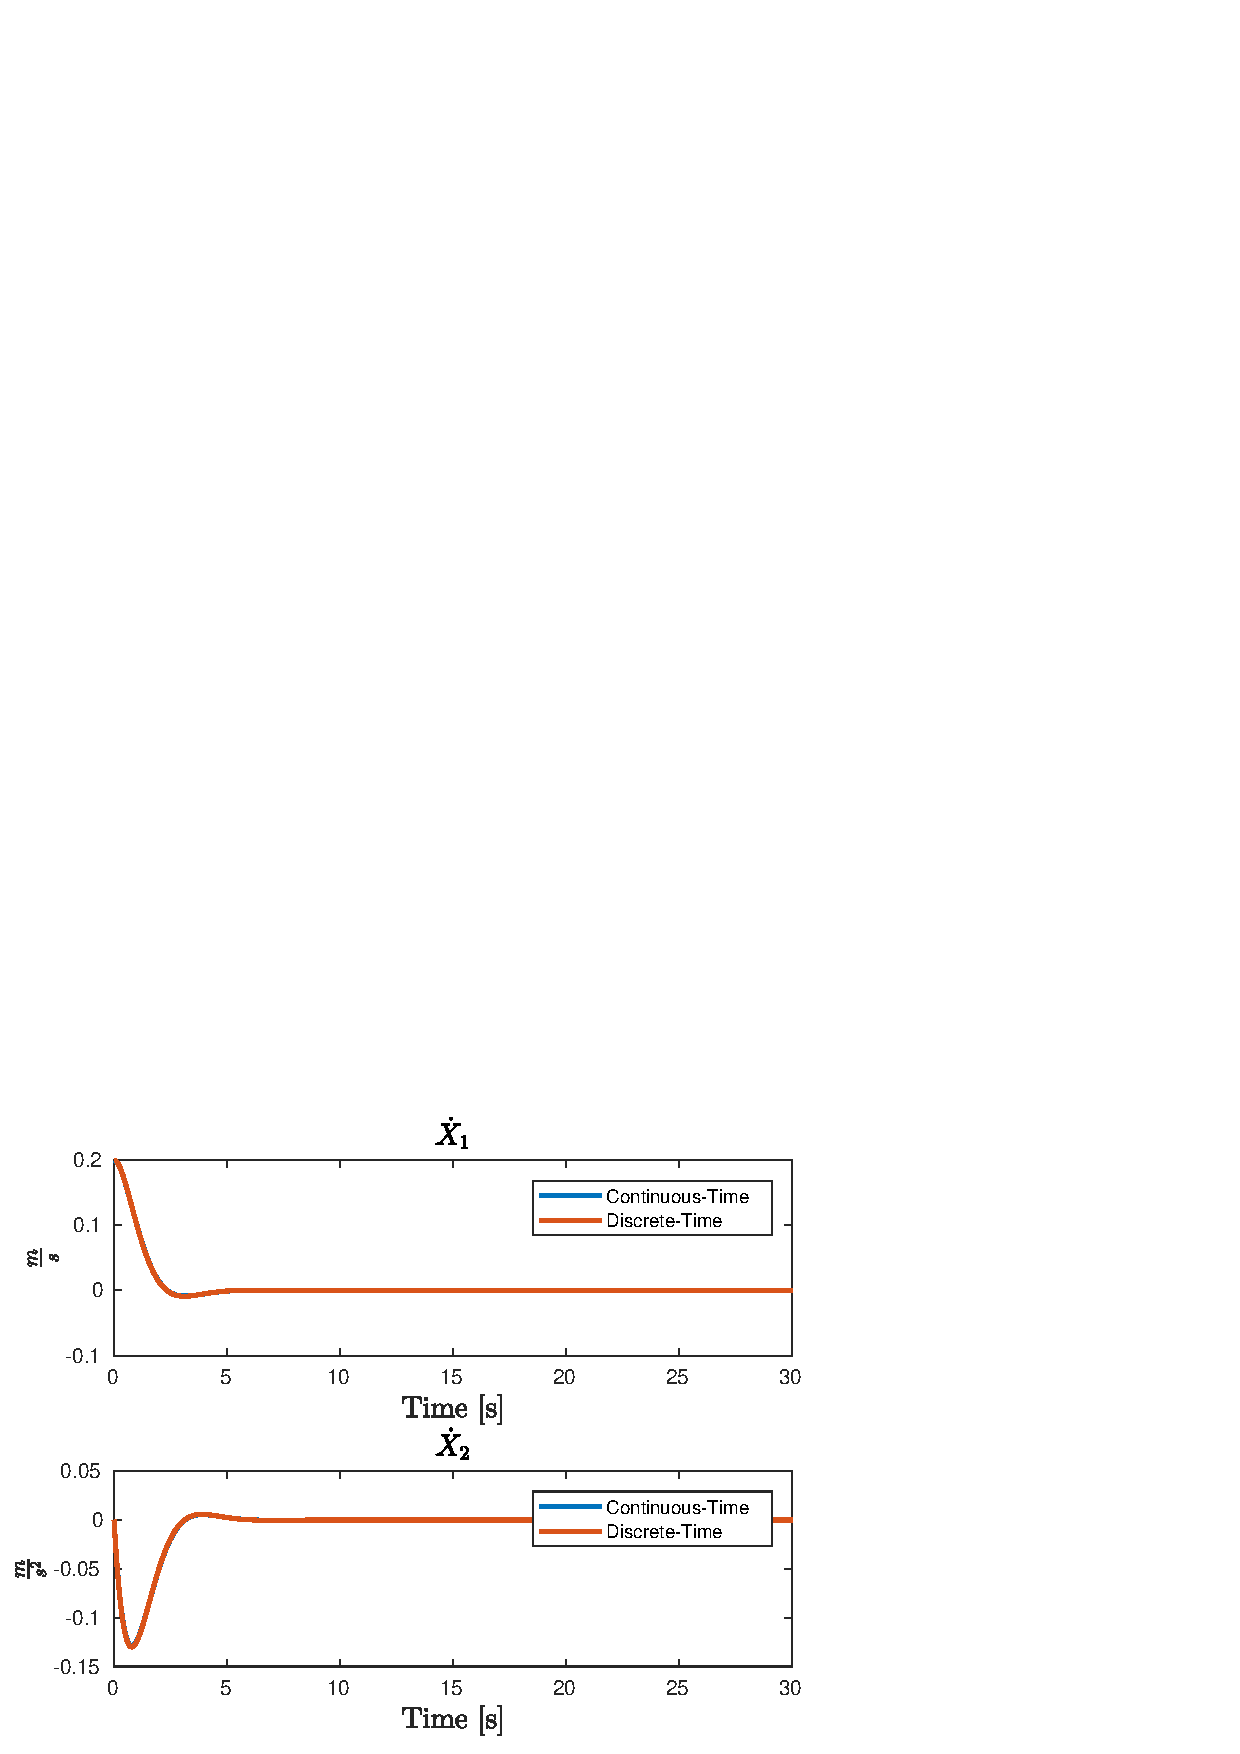
\includegraphics [width=4.5in]{plot1.png}
\caption{Continuous/Discrete Time representation of State Transition Matrix}
\end{figure}  \end{center}

\pagebreak
\textbf{2 } Simulate the discretized system of Kirk Problem 1.3 with a discrete-time LQR with an identity matrix for P(0) and Q.

\textbf{a) } Plot the states for a reasonable time duration and find the magnitude of the largest closed-loop eigenvalue, for R = 0.1, 1, and 10.

\begin{center} \begin{figure} [h]
\includegraphics [width=4.5in]{fig1.pdf}
\caption{Continuous/Discrete Time representation of State Transition Matrix}
\end{figure}  \end{center}

\begin{table}[h]
\centering
\caption{Magnitude of the largest closed-loop eigenvalue}
\label{my-label}
\begin{tabular}{|c|c|}
\hline
\multicolumn{1}{|l|}{\textbf{R}} & \multicolumn{1}{l|}{\textbf{Magnitude Eigenvalue}} \\ \hline
0.1                              & 0.4264                                             \\ \hline
1.0                              & 1.0000                                             \\ \hline
10                               & 1.3484                                             \\ \hline
\end{tabular}
\end{table}

\pagebreak
\textbf{b }Explain how and why the value of R affects the system response and the closed-loop eigenvalues.

	When R increases the magnitude of control effort decreases as represented in the following figure. We can also come up with this statement after observing the performance measure equation. As R increases, the cost function has greater intention on decrease the magnitude of \textit{u}. Also, through R, we can observe that it makes the system less stable because it is getting further outside the unit circle. 

\begin{figure}[h]
\centering
\includegraphics [width=3.9in]{fig4.pdf}
\includegraphics [width=3.9in]{fig5.pdf}
\end{figure}


\pagebreak

\textbf{c) }For R = 1, plot the elements of the state feedback matrix as a function of time.

\begin{figure}[h]
    \centering
	\includegraphics [width=4.5in]{SFMfix.png}
	\caption{Continuous/Discrete Time representation of State Transition Matrix}
\end{figure}

\textbf{d)	}Use the steady-state state feedback matrix (for R = 1) in your controller. How does system performance change relative to time-varying feedback control?

The system has the same response as the time-varying feedback control for the initial conditions $ [0.2; 0]^T$ . It boils down to the fact that during the time-varying feedback control it reach the value of steady-state really fast, less the a 0.1s. We can see in the figure 5 that the control input has an insignificant difference when it is reaching the 30s. Also, we can see in figure 7 that the state feedback matrix \textit{F} found using the Ricatti equation solver in matlab (DARE) is the same value as the \textit{F} for Time-Varying Feedback controller. 

\begin{figure}[p]
\centering
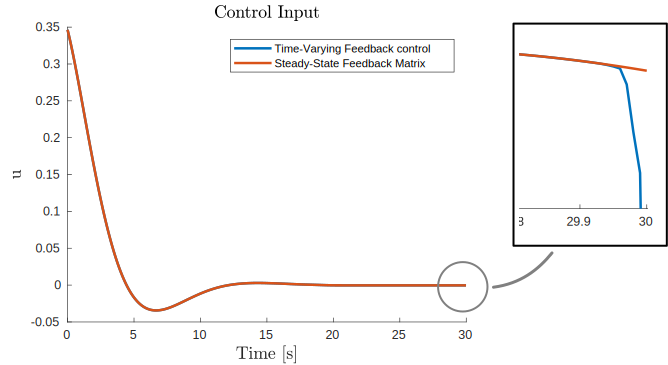
\includegraphics [width=3.8in]{control_input.png}
\caption{Continuous/Discrete Time representation of State Transition Matrix}
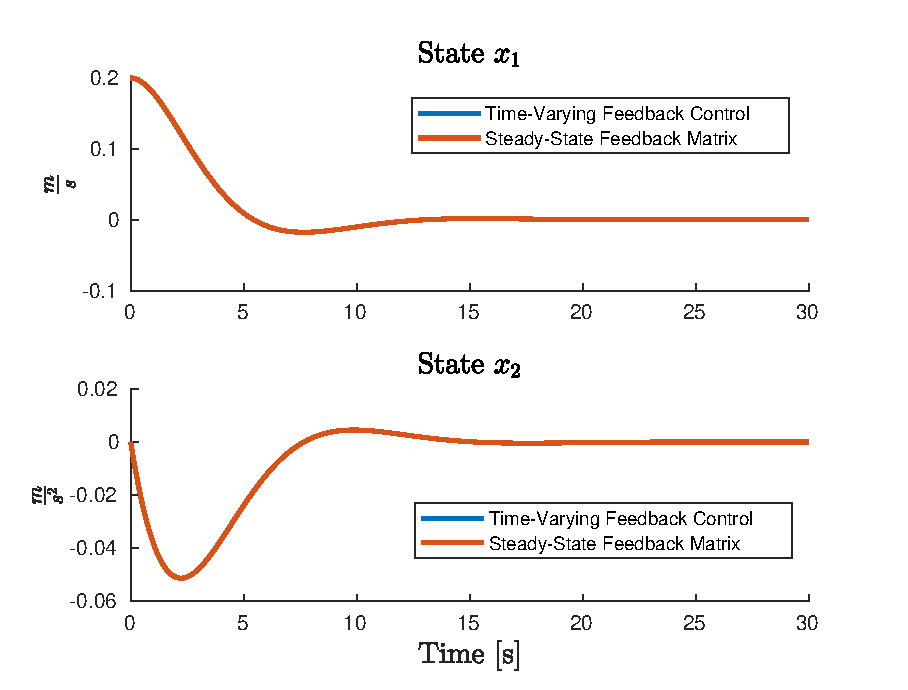
\includegraphics [width=3.8in]{plot2e1.eps}
\includegraphics [width=3.8in]{plot2e2.eps}
\caption{State Feedback Matrix for both cases.}
\end{figure}

\pagebreak

\begin{lstlisting}
% Book: Optimal Control Theory: An Introduction by Donald E. Kirk
%
% Erivelton Gualter, 02/01/2018

clear all; close all;

% Mechanical System Description
M = 1; % kg
K = 2; % N/m
B = 2; % N/m/s

A = [ 0 1; -K/M -B/M];
B = [0 ; 1/M];

% Simulation Parametes
X0 = [0.2; 0];  % Initial States
tf = 30;        % Final time [s]
dt = 1e-2;      % Sampling time
N = tf/dt+3;
t = 0:dt:tf;

% Initialized parameters
P(:,:,1)= eye(size(A));
Q       = eye(size(A));
R_array = [0.1 1 10 1];

% Plots creation
f0 = figure;
f1 = figure;
f2 = figure;
f3 = figure;
f4 = figure;
f5 = figure;
f6 = figure;

figure(f0);
ax1 = subplot(211);
ax2 = subplot(212);

% Analytical solutions
syms s;
xt = ilaplace(inv(s*eye(size(A))-A)*X0);
xta =  [(exp(-t).*(cos(t) + sin(t)))/5;
         -(2*exp(-t).*sin(t))/5];

% Simulate systen
x(1,:) = X0;
for k=1:N-2
    if k ~= 1
        x(k,:) = x_new;
    end

    u(k,:) = 0;
    xdot(k,1) = x(k,2);
    xdot(k,2) = -2*x(k,1) -2*x(k,2) + u(k); 

    x_new = x(k,:) + xdot(k,:)*dt;
end
    figure(f1)
    hold(ax1,'on'); plot(ax1, t, x(:,1), t, xta(1,:), 'LineWidth',2); hold(ax1,'off')
    hold(ax2,'on'); plot(ax2, t, x(:,2), t, xta(2,:), 'LineWidth',2); hold(ax2,'off')
    title(ax1, 'State Transition Matrix to evaluate discretization','Interpreter','latex','FontSize',14); 
    legend(ax1, ['Continuos-Time'], ['Discrete-Time']);
    legend(ax2, ['Continuos-Time'], ['Discrete-Time']);
    xlabel('Time [s]', 'Interpreter','Latex', 'FontSize',14);
    ylabel(ax1,'State $x_1$ $ \frac{m}{s}$', 'Interpreter','Latex', 'FontSize',14);
    ylabel(ax2,'State $x_2$ $ \frac{m}{s^2}$', 'Interpreter','Latex', 'FontSize',14);
    saveFigureToPdf('fig0',f0);
    
%%
figure(f1);
ax3 = subplot(211);
ax4 = subplot(212);

% For for differents R. | e.g. R_array = [0.1 1 10];
for i=1 : length(R_array)
    R = R_array(i);     % set R
    
    % Backwards loop to find P and K
    for k=2:N-1
        S = R + B'*P(:,:,k-1)*B;
        F(:,:,N-k) =  -( inv(S) * B' * P(:,:,k-1) * A );
        P(:,:,k) = (A + B*F(:,:,N-k))'*P(:,:,k-1)*(A + B*F(:,:,N-k)) + F(:,:,N-k)'*R*F(:,:,N-k) + Q;
    end

    % Simulate systen
    x(1,:) = X0;
    for k=1:N-2
        if k ~= 1
            x(k,:) = x_new;
        end
        
        if i==length(R_array)
            Pss = dare(A,B,Q,R);
            S = R + B'*Pss*B;
            Fss = -( inv(S) * B' * Pss * A );
            
            u(k,:) = Fss*x(k,:).';
            
            F = Fss.*ones(size(F));
        else
            u(k,:) = F(:,:,k)*x(k,:).';
        end

        xdot(k,1) = x(k,2);
        xdot(k,2) = -2*x(k,1) -2*x(k,2) + u(k); 

        x_new = x(k,:) + xdot(k,:)*dt;
    end
    
    % Performance Measure (calc cost)
    for k=1:N-2
        J(k) = (x(end,:)*P(:,:,1)*x(end,:)' + x(k,:)*Q*x(k,:)' + u(k,:)*R*u(k,:)')/2;
    end

    % Find MMagnitude of the largest closed-loop eigenvalue
%     for ii = length(x(:,1))
%         cl_sys = A+B*F(:,:,ii);
%         max_eigs(ii,:) = max(abs(eig(cl_sys)));
%     end
%     max_eigen = max(max_eigs)
               
    %% Plots
    figure(f1)
    hold(ax3,'on'); plot(ax3, t, x(:,1),'LineWidth',2); hold(ax3,'off')
    hold(ax4,'on'); plot(ax4, t, x(:,2),'LineWidth',2); hold(ax4,'off')
    title(ax3, 'State $x_1$','Interpreter','latex','FontSize',14); 
    title(ax4, 'State $x_2$','Interpreter','latex','FontSize',14);   
    legend(ax3, ['R = ' num2str(R_array(1))], ['R = ' num2str(R_array(2))], ['R = ' num2str(R_array(3))], ['R = ' num2str(R_array(end)), ' SS']);
    legend(ax4, ['R = ' num2str(R_array(1))], ['R = ' num2str(R_array(2))], ['R = ' num2str(R_array(3))], ['R = ' num2str(R_array(end)), ' SS']);
    xlabel('Time [s]', 'Interpreter','Latex', 'FontSize',14);
    ylabel(ax3,'$ \frac{m}{s}$', 'Interpreter','Latex', 'FontSize',14);
    ylabel(ax4,'$ \frac{m}{s^2}$', 'Interpreter','Latex', 'FontSize',14);
    saveFigureToPdf('fig1',f1);

    figure(f2); hold on; 
    F_plot(:,:) = F(1,:,:); plot(t,F_plot,'LineWidth',2);
    legend(['R = ' num2str(R_array(1))], ['R = ' num2str(R_array(1))], ['R = ' num2str(R_array(2))], ['R = ' num2str(R_array(2))],['R = ' num2str(R_array(3))],['R = ' num2str(R_array(3))]);
    title('State Feedback Matrix $F$','Interpreter','latex','FontSize',14); 
    xlabel('N', 'Interpreter','Latex', 'FontSize',14);
    ylabel('F', 'Interpreter','Latex', 'FontSize',14);
    saveFigureToPdf('fig2',f2);

    figure(f3); hold on
    F_plot(:,:) = F(1,:,:); plot(t,F_plot,'LineWidth',2);
    xlim([max(t)-1 max(t)]);
    legend(['R = ' num2str(R_array(1))], ['R = ' num2str(R_array(1))], ['R = ' num2str(R_array(2))], ['R = ' num2str(R_array(2))],['R = ' num2str(R_array(3))],['R = ' num2str(R_array(3))]);
    title('State Feedback Matrix $F$','Interpreter','latex','FontSize',14); 
    xlabel('N', 'Interpreter','Latex', 'FontSize',14);
    ylabel('F', 'Interpreter','Latex', 'FontSize',14);
    saveFigureToPdf('fig3',f3);

    figure(f4); hold on
    plot(t,u,'LineWidth',2);
    legend(['R = ' num2str(R_array(1))], ['R = ' num2str(R_array(1))], ['R = ' num2str(R_array(2))], ['R = ' num2str(R_array(2))],['R = ' num2str(R_array(3))],['R = ' num2str(R_array(3))]);
    title('Control Input','Interpreter','latex','FontSize',14); 
    xlabel('Time [s]', 'Interpreter','Latex', 'FontSize',14);
    ylabel('u', 'Interpreter','Latex', 'FontSize',14);
    saveFigureToPdf('fig4',f4);
    
    figure(f5); hold on
    plot(t, J, 'LineWidth', 2)
    legend(['R = ' num2str(R_array(1))], ['R = ' num2str(R_array(2))], ['R = ' num2str(R_array(3))], ['R = ' num2str(R_array(end)), ' SS']);
    title('Performance Measure LQR (Cost Function)','Interpreter','latex','FontSize',14); 
    xlabel('Time [s]', 'Interpreter','Latex', 'FontSize',14);
    ylabel('Cost Function', 'Interpreter','Latex', 'FontSize',14);
    saveFigureToPdf('fig5',f5);
    
    clear P F
    P(:,:,1)= eye(size(A));
end
\end{lstlisting}

You can access the code at: https://github.com/EriveltonGualter/EEC-744-Optimal-Control-Systems



\end{document}
